\documentclass{article}

\usepackage[utf8]{inputenc}
\usepackage{amsthm}
\usepackage{amsmath}

\usepackage{graphicx}

\usepackage{french}

\usepackage{listings}
\lstset{language=R}

\begin{document}

\tableofcontents

\newpage

\section{Série Temporelle - La Théorie}

\subsection{Auto-Régression (AR)}

\subsubsection{Définition}
Un processus $(X_t)$ est Auto-Régressif quand sa valeur à l'instant t n'est expliquée que par ses anciennes valeurs $(X_{t-1},...,X_{t-i})$, où $i\in\{2,...,\infty\}$ et non par d'autres processus.
$$X_t=\phi_1{X_{t-1}}+...+\phi_i{X_{t-i}}+\epsilon_t, \quad i\in\{2,...,\infty\},$$
où les $\epsilon_t$ sont des bruits blancs, indépendants et identiquement distribués, notés $\epsilon_t \rightarrow iid(0,\sigma^2), \; \forall t$.

\subsubsection{Ordre d'un AR}
Un processus AR est d'ordre p, noté AR(p), quand sa valeur à l'instant t est expliquée par ses p anciennes valeurs: 
$$X_t=\phi_1{X_{t-1}}+...+\phi_p{X_{t-p}}+\epsilon_t,$$
où $\epsilon_t \rightarrow iid(0,\sigma^2), \; \forall t$.

\subsubsection{Opérateur de retard}
Pour une série temporelle $(X_t)_t$, on définit l'opérateur de retard, noté L, par une application qui à chaque élément $X_t$ de la série, associe son observation précédente $X_{t-1}$:
$$LX_t=X_{t-1}, \quad \forall t>1.$$
En particulier, $L^i(X_t)=X_{t-i}$.

\subsubsection{Opérateur de différenciation}
Pour une série temporelle $(X_t)_t$, on définit l'opérateur de différenciation, noté $\nabla$, par une application qui à chaque élément $X_t$ de la série, associe la différence $X_t-X_{t-1}$:
$$\nabla{X_t}=X_t-X_{t-1}, \quad \forall t>1.$$

\subsubsection{Polynôme caractéristique}
Ayant définit l'opérateur de retard, on peut l'utiliser dans la définition d'un processus AR(p).
\newline
Ainsi, si $(X_t)_t$ est un AR(p), alors, on définit le polynôme caractéristique $\Phi$ d'un processus AR(p) de tel sorte que: $\Phi(L){X_t}=\epsilon_t$,
$$\Phi(L)=1-\phi_1{L^1}+...+\phi_p{L^p}.$$

\subsubsection{Équation caractéristique}
On appelle équation caractéristique d'un processus AR(p), l'équation déduit de $\Phi$ en remplaçant L par x:
$$(1-\phi_1{x^1}+...+\phi_p{x^p}).$$

\subsection{Moyenne Mobile (MA)}

\subsubsection{Introduction}
Une moyenne est dite mobile lorsqu'elle est recalculée de façon continue, en utilisant à chaque calcul un sous-ensemble d'éléments dans lequel un nouvel élément remplace le plus ancien ou s'ajoute au sous-ensemble.

\subsubsection{Définition}
Un processus est une Moyenne Mobile lorsqu'il est de la forme:
$$X_t=\theta_1{\epsilon_{t-1}}+...+\theta_i{\epsilon_{t-i}}+\epsilon_t, \quad i\in\{2,...,\infty\},$$
où $\epsilon_t \rightarrow iid(0,\sigma^2), \; \forall t$.

\subsubsection{Ordre d'un MA}
Un processus MA est d'ordre q, noté MA(q), quand sa valeur à l'instant t est expliquée par ses q anciennes valeurs: 
$$X_t=\theta_1{\epsilon_{t-1}}+...+\theta_p{\epsilon_{t-q}}+\epsilon_t,$$
où $\epsilon_t \rightarrow iid(0,\sigma^2), \; \forall t$.

\subsubsection{Polynôme caractéristique}
Le polynôme caractéristique $\Theta$ d'un processus MA(q) est definit de tel sorte que: $X_t=\Theta(L)\epsilon_t$,
$$\Theta(L)=1+\theta_1{L^1}+...+\theta_q{L^q}.$$

\subsection{Auto-Regression et Moyenne Mobile (ARMA)}

\subsubsection{Définition}
Un processus ARMA $(X_t)_t$ est comme son nom l'indique, un processus auto-regéssif et moyenne mobile. Il a une partie AR(p) et une partie MA(q) et est noté ARMA(p,q) selon la définition:
$$X_t:=\phi_1{X_{t-1}}+...+\phi_p{X_{t-p}}+\theta_1{\epsilon_{t-1}}+...+\theta_p{\epsilon_{t-q}}+\epsilon_t,$$
où $\epsilon_t \rightarrow iid(0,\sigma^2), \; \forall t$.

\subsubsection{Stationnarité faible}
Un processus $(X_t)_t$ est faiblement stationnaire si: $\forall t$, $\forall h<t$;
\begin{itemize}
\item $E(X_t)=\mu$, l'espérence est constante au cours du temps.
\item $Var(X_t)=\sigma^2<\infty$, la variance est constante et non infinie.
\item $Cov(X_t,X_{t-h})=\gamma(h)$, l'auto-corrélation entre $X_t$ et $X_{t-h}$ reste constante et ne dépend que de h.
\end{itemize}

\subsubsection{Stationnarité forte}
Un processus $(X_t)_t$ est fortement stationnaire si: $\forall t$, $\forall h$; $(X_1,X_2,...,X_t)$ et $(X_{1+h},X_{2+h},...,X_{t+h})$ ont même lois en probabilité.

\subsubsection{Auto-Corrélation (ACF)}
La fonction d'auto-corrélation $\rho$ est définie par:
$$\rho(h)=\frac{\gamma(h)}{\gamma(0)}=\frac{E[(X_t-\mu)(X_{t+h}-\mu)]}{\sigma^2}.$$

\subsubsection{ACF et Ordre de la MA}
Si on observe le graphe de l'ACF, le dernier pic significatif nous donnera l'ordre q de la partie MA du processus.

\subsubsection{Auto-Corrélation Partielle (PACF)}
La fonction d'auto-corrélation partielle $L$ est définie par:
\begin{align*}
L(0)&=1,\\
L(h)&=\phi_{hh}, \; \forall h>0,
\end{align*}
avec $\phi_h={\Gamma^{-1}_h}{\gamma_h}$, $\Gamma_h=(\gamma(i-j))_{1\leq{i,j}\leq{h}}$, $\gamma_h=(\gamma(1),\gamma(2),...,\gamma(h))$.

\subsubsection{PACF et Ordre de l'AR}
Si on observe le graphe de la PACF, le dernier pic significatif nous donnera l'ordre p de la partie AR du processus.

\subsection{Auto-Regression, Integrée et Moyenne Mobile (ARIMA)}
\subsubsection{Définition}
Les modèles ARIMA sont des modèles qui se réduisent à des ARMA une fois différentiés un nombre fini de fois. On a alors la notation ARIMA(p,d,q), où 
\begin{itemize}
\item p: ordre de la partie AR,
\item d: ordre de différentiation,
\item q: ordre de la partie MA.
\end{itemize}

\subsubsection{Définition 2}
Un modèle ARIMA(p,d,q) est de la forme:
$$A(L)(1-L)^d{X_t}=B(L)\epsilon_t,$$
où A(L) et B(L) sont les polynômes caractéristiques respectives des parties AR et MA.

\subsection{Tests avec les séries temporelles}

\subsubsection{p-value}
En  statistique, le p-value est une critère d'acceptation de l'hypothèse nulle $(H_0)$:
\begin{itemize}
\item si p-value$>0.05$, $(H_0)$ est acceptée,
\item si p-value$\leq0.05$, $(H_0)$ est rejetée.
\end{itemize}

\subsubsection{Test de Dickey-Fuller Augmenté - ADF}
Le test ADF est un test de racine unitaire:
\newline
$(H_0):$ Le processus admet une racine unitaire (non stationnaire), contre
\newline
$(H_1):$ Le processus est stationnaire.

\subsubsection{Test de Box-Pierce}
Le Test de Box-Pierce est un test statistique qui teste l'auto-corrélation:
\newline
$(H_0):$ Aucune corrélation dans les erreurs, contre
\newline
$(H_1):$ Avec corrélation dans les erreurs.
\newpage

\section{Série Temporelle - La Pratique}

\subsection{Introduction}
En analyse théorique, l'étude d'une série temporelle commence par sa forme théorique. Par exemple, l'étude d'un processus ARMA(p,q) $(X_t)_t$ débute par sa forme:
$$X_t=\phi_1{X_{t-1}}+...+\phi_p{X_{t-p}}+\theta_1{\epsilon_{t-1}}+...+\theta_p{\epsilon_{t-q}}+\epsilon_t,$$
où les $\phi_i$ et $\theta_j$ sont des constantes données $\forall i<p, \; \forall j<q$.
\newline

Par contre, l'analyse pratique d'une série temporelle débute par un tableau de données, et grâce à ces données, on essaie d'estimer les paramètres du processus, et de déterminer les propriétés des résidus.

\subsection{Les données}
Pour cette analyse, nous allons étudier les variations annuelles de la quantité d'émission de $C0_2$ à Madagascar de 1960 à 2011.

\begin{figure}[h!]
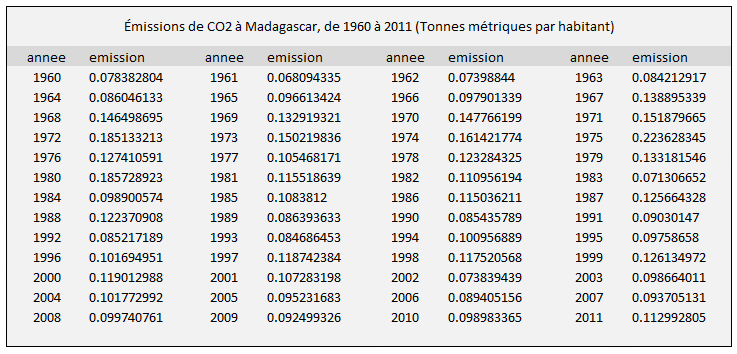
\includegraphics[width=\linewidth]{images/data.png}
\caption{Tonnes métriques d'émission de CO2 à Madagascar}
\label{fig:data}
\end{figure}

\newpage

\subsection{La serie temporelle}
La serie temporelle $(Y_t)$ obtenue à partir de ces données produit la graphe ci-dessous.
\begin{figure}[h!]
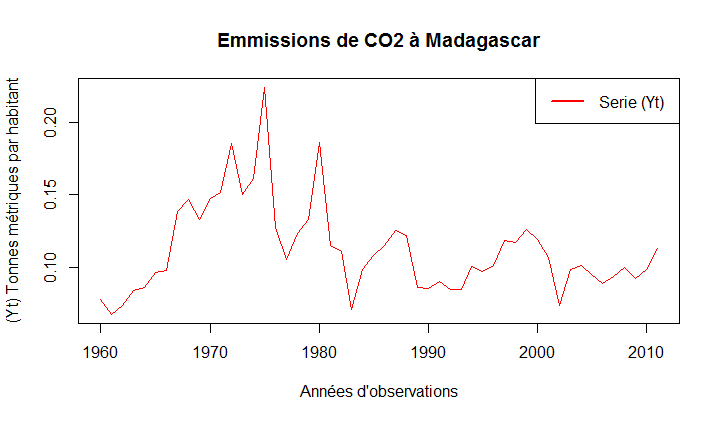
\includegraphics[width=\linewidth]{images/Yt.png}
\caption{Graphe, Tonnes métriques d'émission de CO2 à Madagascar}
\label{fig:Yt}
\end{figure}

De plus, elles produisent les graphes des ses corrélogrammes ci-dessous.
\begin{figure}[h!]
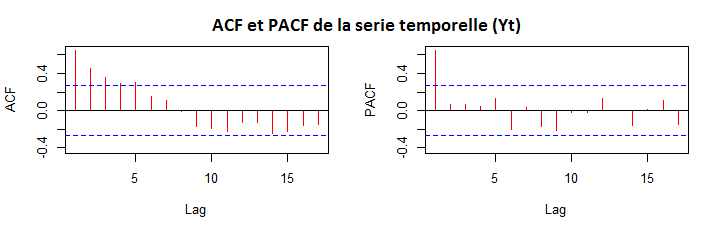
\includegraphics[width=\linewidth]{images/Yt_acf_pacf.png}
\caption{Graphe, Tonnes métriques d'émission de CO2 à Madagascar}
\label{fig:Yt_acf_pacf}
\end{figure}

\subsubsection{Identification de la série}
On peut constater à partir des corrélogrammes que:
\begin{itemize}
\item l'ACF donne q=5, ainsi on a MA(5), et
\item la PACF donne p=1, alors on a AR(1),
\end{itemize}
donc, si les résidus sont iid, alors la série $(Y_t)$ est ARMA(1,5).

\subsubsection{Stationnarité de la série}
Le Test de Dickey-Fuller Augmenté nous donne les résultats suivants:

\begin{figure}[h!]
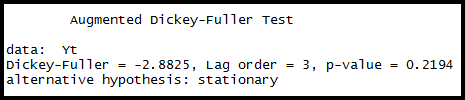
\includegraphics[width=\linewidth]{images/Yt_adf.png}
\caption{Test de Dickey-Fuller sur la série (Yt)}
\label{fig:Yt_adf}
\end{figure}

On constate ici que le p-value = 0.2194, ne nous permet pas de rejetter l'hypothèse nulle $(H_0)$, ainsi, la série $(Y_t)$ n'est PAS STATIONNAIRE.

\subsection{La série temporelle differenciée}
Continuons notre étude, mais utilisons cette fois ci la série différentiée (diff{\_}$Y_t$) de $(Y_t)$. On a alors sa graphe, ainsi que ses deux corrélogrammes, simple et partiel: 

\begin{figure}[h!]
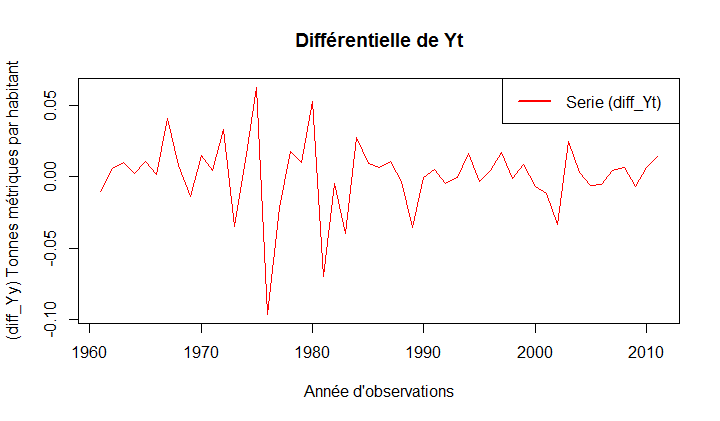
\includegraphics[width=\linewidth]{images/diff_Yt.png}
\caption{Graphe de la serie (diff{\_}$Y_t$)}
\label{fig:diff_Yt}
\end{figure}

\begin{figure}[h!]
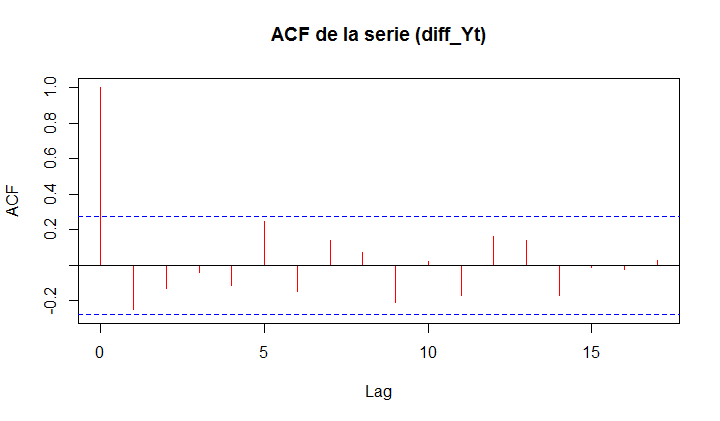
\includegraphics[width=\linewidth]{images/diff_Yt_acf.png}
\caption{L'ACF de la serie (diff{\_}$Y_t$)}
\label{fig:diff_Yt_acf}
\end{figure}

\begin{figure}[h!]
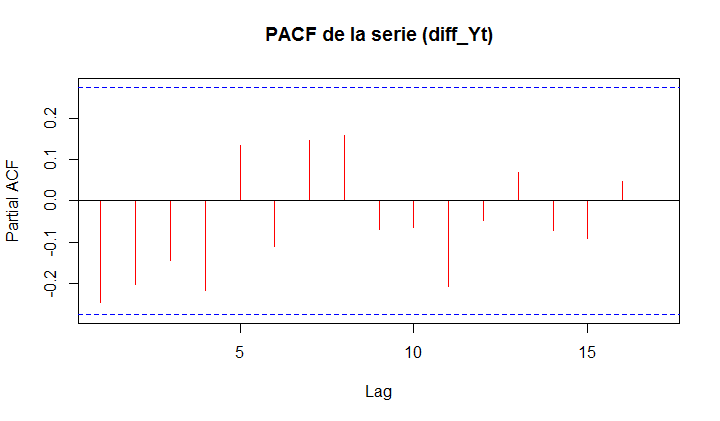
\includegraphics[width=\linewidth]{images/diff_Yt_pacf.png}
\caption{La PACF de la série (diff{\_}$Y_t$)}
\label{fig:diff_Yt_pacf}
\end{figure}

\newpage

\subsubsection{Identification de la série différentiée}
On peut constater à partir des corrélogrammes que:

\begin{itemize}
\item l'ACF donne q=1, ainsi on a MA(1), et
\item la PACF donne p=0, alors on a AR(0),
\end{itemize}

donc, si les résidus sont iid, alors la série (diff{\_}$Y_t$) est un processus ARMA(0,1) ou plus précisément un MA(1).

\subsubsection{Stationnarité de la série différentiée}
Le Test de Dickey-Fuller Augmenté nous donne les résultats suivants:

\begin{figure}[h!]
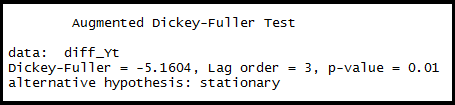
\includegraphics[width=\linewidth]{images/diff_Yt_adf.png}
\caption{Test de Dickey-Fuller sur la série (diff{\_}$Y_t$)}
\label{fig:diff_Yt_adf}
\end{figure}

On constate ici que le p-value = 0.01, nous incite à rejeter l'hypothèse nulle $(H_0)$, ainsi, la série (diff{\_}$Y_t$) est STATIONNAIRE.

\subsection{Les Résidus}
On a donc une série temporelle différentiée (diff{\_}$Y_t$) stationnaire, avec les ordres:
\begin{itemize}
\item p=0, d'après la PACF,
\item d=1, l'ordre de différenciation, 
\item q=1, d'après l'ACF.
\end{itemize}

Ainsi, on a un processus ARIMA(0,1,1) si les résidus de cette série sont des bruits blanc.

\newpage

\subsubsection{Propriétés des résidus}
Les figures ci-dessous sont le graphe et les corrélogrammes simple et partielles des residus du processus issus de $(Y_t)$ et des études précédents.

\begin{figure}[h!]
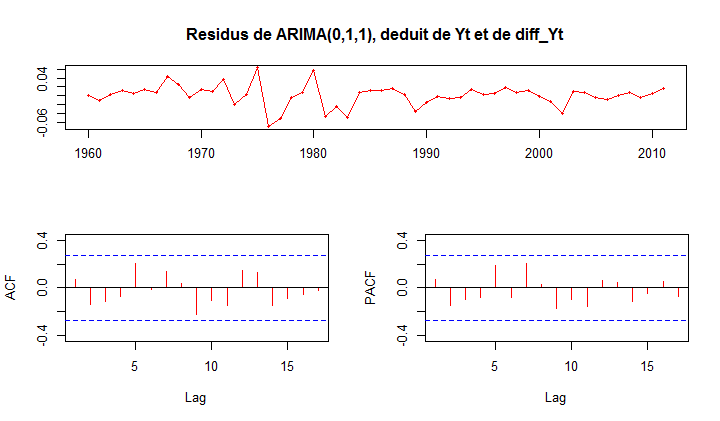
\includegraphics[width=\linewidth]{images/Yt_residus.png}
\caption{Graphe, ACF et PACF des résidus}
\label{fig:Yt_residus}
\end{figure}

On observe alors qu'il n'y a aucun pic significatif dans les corrélogrammes des résidus.

De plus, le test de Box-Pierce appliqué aux résidus nous donne:

\begin{figure}[h!]
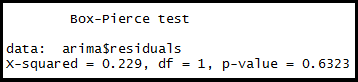
\includegraphics[width=\linewidth]{images/Yt_residus_bp.png}
\caption{Test de Box-Pierce sir les résidus}
\label{fig:Yt_residus_bp}
\end{figure}

On en déduit donc que les résidus sont des bruits blancs et, par conséquent le processus issus de $(Y_t)$ et de notre étude est bien un ARIMA(0,1,1).

\subsection{Le modèle}
Notre étude nous a permis de constater que: $(1-L)^1{Y_t}=(1+\theta{L})\epsilon_t$, puisque
\begin{itemize}
\item le modèle est un ARIMA(0,1,1),
\item les résidus sont des bruits blancs.
\end{itemize}
Il nous reste donc à déterminer $\theta$. Or,

\begin{figure}[h!]
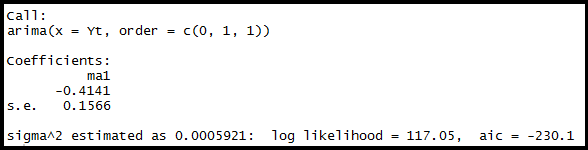
\includegraphics[width=\linewidth]{images/Yt_coeff.png}
\caption{Propriétés du modèle}
\label{fig:Yt_coeff}
\end{figure}

Finalement, le modèle est:

\begin{figure}[h!]
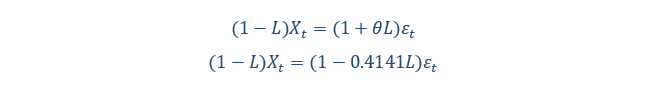
\includegraphics[width=\linewidth]{images/Yt_arima.png}
\end{figure}

\subsection{La prévision}

\begin{figure}[h!]
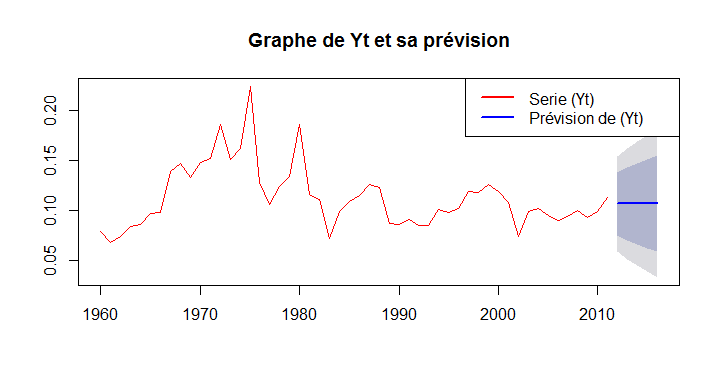
\includegraphics[width=\linewidth]{images/Yt_prevision.png}
\caption{Prévision de la série $(Y_t)$}
\label{fig:Yt_prevision}
\end{figure}

Après avoir vérifié que notre série est bien un ARMA(0,1,1) dont les résidus sont des bruits blancs, on peut trouver une intervalle de prévision pouvant contenir les prochaines valeurs de notre série $(Y_t)$. Ceci est expliqué par le graphe ci-dessus:


\newpage

\subsection{La série ajustée}

\begin{figure}[h!]
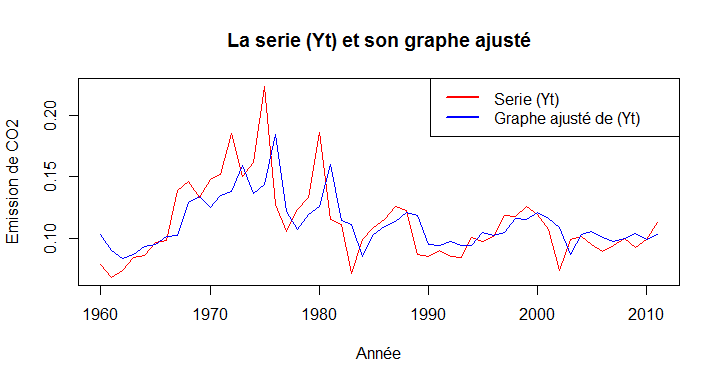
\includegraphics[width=\linewidth]{images/Yt_ajustee.png}
\caption{Graphe ajusté de la série $(Y_t)$}
\label{fig:Yt_ajustee}
\end{figure}

\subsection{La prévision de la série ajustée}
Le graphe ajusté de nous donne une intervalle de prévision selon le graphe suivant:

\begin{figure}[h!]
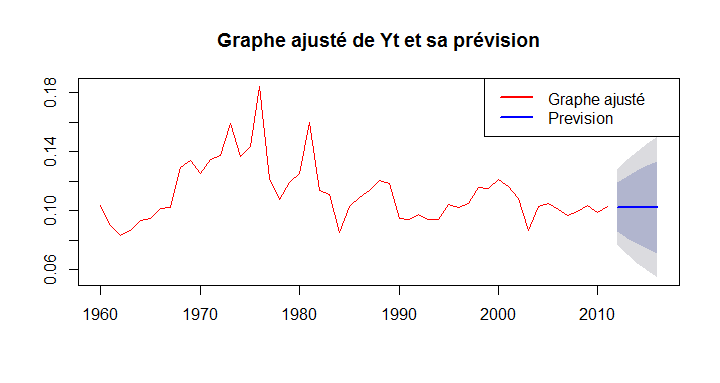
\includegraphics[width=\linewidth]{images/Yt_ajustee_prediction.png}
\caption{Graphe ajusté de la série $(Y_t)$ et sa prédiction}
\label{fig:Yt_ajustee_prediction}
\end{figure}

\end{document}
